\documentclass[12pt]{article}
\usepackage[english]{babel}
\usepackage[utf8]{inputenc}
\usepackage[english]{babel}
\usepackage[a4paper, total={7.25in, 9.5in}]{geometry}
\usepackage{tikz-feynman}
\tikzfeynmanset{compat=1.0.0} 
\usepackage{subcaption}
\usepackage{float}
\floatplacement{figure}{H}
\usepackage{mathrsfs}  
\usepackage{dsfont}
\usepackage{relsize}
\DeclareMathAlphabet{\mathdutchcal}{U}{dutchcal}{m}{n}

\usepackage{revsymb}


\newcommand{\field}{\hat{\Phi}}
\newcommand{\dfield}{\hat{\Phi}^\dagger}
 
\usepackage{amsthm, amssymb, amsmath, centernot}
\usepackage{slashed}
\newcommand{\notimplies}{%
  \mathrel{{\ooalign{\hidewidth$\not\phantom{=}$\hidewidth\cr$\implies$}}}}
 
\renewcommand\qedsymbol{$\square$}
\newcommand{\cont}{$\boxtimes$}
\newcommand{\divides}{\mid}
\newcommand{\ndivides}{\centernot \mid}

\newcommand{\Integers}{\mathbb{Z}}
\newcommand{\Natural}{\mathbb{N}}
\newcommand{\Complex}{\mathbb{C}}
\newcommand{\Zplus}{\mathbb{Z}^{+}}
\newcommand{\Primes}{\mathbb{P}}
\newcommand{\Q}{\mathbb{Q}}
\newcommand{\R}{\mathbb{R}}
\newcommand{\ball}[2]{B_{#1} \! \left(#2 \right)}
\newcommand{\Rplus}{\mathbb{R}^+}
\renewcommand{\Re}[1]{\mathrm{Re}\left[ #1 \right]}
\renewcommand{\Im}[1]{\mathrm{Im}\left[ #1 \right]}
\newcommand{\Op}{\mathcal{O}}

\newcommand{\invI}[2]{#1^{-1} \left( #2 \right)}
\newcommand{\End}[1]{\text{End}\left( A \right)}
\newcommand{\legsym}[2]{\left(\frac{#1}{#2} \right)}
\renewcommand{\mod}[3]{\: #1 \equiv #2 \: \mathrm{mod} \: #3 \:}
\newcommand{\nmod}[3]{\: #1 \centernot \equiv #2 \: mod \: #3 \:}
\newcommand{\ndiv}{\hspace{-4pt}\not \divides \hspace{2pt}}
\newcommand{\finfield}[1]{\mathbb{F}_{#1}}
\newcommand{\finunits}[1]{\mathbb{F}_{#1}^{\times}}
\newcommand{\ord}[1]{\mathrm{ord}\! \left(#1 \right)}
\newcommand{\quadfield}[1]{\Q \small(\sqrt{#1} \small)}
\newcommand{\vspan}[1]{\mathrm{span}\! \left\{#1 \right\}}
\newcommand{\galgroup}[1]{Gal \small(#1 \small)}
\newcommand{\bra}[1]{\left| #1 \right>}
\newcommand{\Oa}{O_\alpha}
\newcommand{\Od}{O_\alpha^{\dagger}}
\newcommand{\Oap}{O_{\alpha '}}
\newcommand{\Odp}{O_{\alpha '}^{\dagger}}
\newcommand{\im}[1]{\mathrm{im} \: #1}
\renewcommand{\ker}[1]{\mathrm{ker} \: #1}
\newcommand{\ket}[1]{\left| #1 \right>}
\renewcommand{\bra}[1]{\left< #1 \right|}
\newcommand{\inner}[2]{\left< #1 | #2 \right>}
\newcommand{\expect}[2]{\left< #1 \right| #2 \left| #1 \right>}
\renewcommand{\d}[1]{\: \mathrm{d}#1 \:}
\newcommand{\dn}[2]{ \mathrm{d}^{#1} #2 \:}
\newcommand{\deriv}[2]{\frac{\d{#1}}{\d{#2}}}
\newcommand{\nderiv}[3]{\frac{\dn{#1}{#2}}{\d{#3^{#1}}}}
\newcommand{\pderiv}[2]{\frac{\partial{#1}}{\partial{#2}}}
\newcommand{\fderiv}[2]{\frac{\delta #1}{\delta #2}}
\newcommand{\parsq}[2]{\frac{\partial^2{#1}}{\partial{#2}^2}}
\newcommand{\topo}{\mathcal{T}}
\newcommand{\base}{\mathcal{B}}
\renewcommand{\bf}[1]{\mathbf{#1}}
\renewcommand{\a}{\hat{a}}
\newcommand{\adag}{\hat{a}^\dagger}
\renewcommand{\b}{\hat{b}}
\newcommand{\bdag}{\hat{b}^\dagger}
\renewcommand{\c}{\hat{c}}
\newcommand{\cdag}{\hat{c}^\dagger}
\newcommand{\hamilt}{\hat{H}}
\renewcommand{\L}{\hat{L}}
\newcommand{\Lz}{\hat{L}_z}
\newcommand{\Lsquared}{\hat{L}^2}
\renewcommand{\S}{\hat{S}}
\renewcommand{\empty}{\varnothing}
\newcommand{\J}{\hat{J}}
\newcommand{\lagrange}{\mathcal{L}}
\newcommand{\dfourx}{\mathrm{d}^4x}
\newcommand{\meson}{\phi}
\newcommand{\dpsi}{\psi^\dagger}
\newcommand{\ipic}{\mathrm{int}}
\newcommand{\tr}[1]{\mathrm{tr} \left( #1 \right)}
\newcommand{\C}{\mathbb{C}}
\newcommand{\CP}[1]{\mathbb{CP}^{#1}}
\newcommand{\Vol}[1]{\mathrm{Vol}\left(#1\right)}

\newcommand{\Tr}[1]{\mathrm{Tr}\left( #1 \right)}
\newcommand{\Charge}{\hat{\mathbf{C}}}
\newcommand{\Parity}{\hat{\mathbf{P}}}
\newcommand{\Time}{\hat{\mathbf{T}}}
\newcommand{\Torder}[1]{\mathbf{T}\left[ #1 \right]}
\newcommand{\Norder}[1]{\mathbf{N}\left[ #1 \right]}
\newcommand{\Znorm}{\mathcal{Z}}
\newcommand{\EV}[1]{\left< #1 \right>}
\newcommand{\interact}{\mathrm{int}}
\newcommand{\covD}{\mathcal{D}}
\newcommand{\conj}[1]{\overline{#1}}

\newcommand{\SO}[2]{\mathrm{SO}(#1, #2)}
\newcommand{\SU}[2]{\mathrm{SU}(#1, #2)}

\newcommand{\anticom}[2]{\left\{ #1 , #2 \right\}}


\newcommand{\pathd}[1]{\! \mathdutchcal{D} #1 \:}

\renewcommand{\theenumi}{(\alph{enumi})}


\renewcommand{\theenumi}{(\alph{enumi})}

\newcommand{\atitle}[1]{\title{% 
	\large \textbf{ASTR GR6001 Radiative Processes
	\\ Assignment \# #1} \vspace{-2ex}}
\author{Benjamin Church }
\maketitle}

\theoremstyle{definition}
\newtheorem{theorem}{Theorem}[section]
\newtheorem{definition}{definition}[section]
\newtheorem{lemma}[theorem]{Lemma}
\newtheorem{proposition}[theorem]{Proposition}
\newtheorem{corollary}[theorem]{Corollary}
\newtheorem{example}[theorem]{Example}
\newtheorem{remark}[theorem]{Remark}
 


\begin{document}

\atitle{2}

\newcommand{\Inumax}{I_\nu^{\text{max}}}
\usetikzlibrary{quotes,angles}


\section*{Problem 1}
Suppose the sun has a limb-darkening law of the form,
\[ I_\nu(\mu) = \Inumax [1 - a(1 - \mu)] \]
Then, at the surface,
\begin{align*}
F_\nu^{\text{surf}} & = \int_{\text{out}}  \mu I_\nu(\mu) \d{\Omega} = 2 \pi \Inumax \int_0^{1} \mu [1 - a(1 - \mu)] 
 \\
 & = 2 \pi \Inumax  [ \tfrac{1}{2} - a ( \tfrac{1}{2} - \tfrac{1}{3})]
\\
& =  \pi \Inumax  [ 1 - \tfrac{1}{3}a ] 
\end{align*} 
Now, consider the flux throught a surface on the earth at a distance $d$ from the sun. Consider the following triangle,
\begin{center}
\begin{tikzpicture}
  \draw
  (0,0) coordinate (a) node[left] {$\bigodot$}
  -- (6, 0) node[anchor=north] {$d$} -- (12,0) coordinate (b) node[right] {$\bigoplus$}
  -- (2,2) coordinate (c) node[above right] {surf.} 
  -- (1,1) node[left] {$r$} -- cycle
    pic["$\alpha$",draw=black,<->,angle eccentricity=1.2,angle radius=2cm] {angle=c--b--a}
    pic["$\theta$",draw=black,<->,angle eccentricity=1.5,angle radius=0.5cm] {angle=a--c--b};
    \draw[thick, dashed] (0,0) circle (2.828);
\end{tikzpicture}
\end{center}
By the law of sines,
\[ \frac{d}{\sin{\theta}} = \frac{r}{\sin{\alpha}} \]
Taking derivatives, we find that,
\[ \cos{\alpha} \d{\alpha} = \frac{r}{d} \cos{\theta} \d{\theta} \]
Multiplying these equations together gives,
\[ \cos{\alpha} \sin{\alpha} \d{\alpha} = \left( \frac{r}{d} \right)^2 \cos{\theta} \sin{\theta} \d{\theta} \]
which implies that,
\[ \cos{\alpha} \d{\Omega'} = \left( \frac{r}{d} \right)^2 \cos{\theta} \d{\Omega} \]
Now the flux at the earth is given by the integral,
\[ F_\nu^{\text{earth}} = \int I_\nu(\alpha) \cos{\alpha} \d{\Omega'} \]
since specific intensity is conserved along rays we have $I_\nu(\alpha) = I_\nu(\theta(\alpha))$. Thus,
\[ F_\nu^{\text{earth}} = \int_{\text{out}} I_\nu(\theta) \left( \frac{r}{d} \right)^2 \cos{\theta} \d{\Omega} = \left( \frac{r}{d} \right)^2 \int_{\text{out}} I_\nu(\theta)  \cos{\theta} \d{\Omega} = \left( \frac{r}{d} \right)^2 F_\nu^{\text{surf}}  \]
which is exactly what we ought to expect from the conservation of energy and the observation that, althought the radiation field of the sun is not isotropic, the outward energy flow is spherically symmetric. 


\section*{Problem 2}

For simplicity, we shall assume that the orbit of the earth has zero eccentricity and that the observer is situated far enough from the planetary system that we can approximate the outgoing rays as parallel. Let the orbit of the planet be inclined at an angle $i$ to the observer's line of sight. Then, choosing a coordinate system centered at the star, with the observer in the $\hat{x}$ direction and the planet's velocty along $\hat{y}$ at its closest approach to the observer. We choose the time coordinate to be zero at this point of closest approach. Thus the orbit is described by,
\[ \vec{r} = r_o (\cos{(\Omega t)} \cos{i}, \sin{(\Omega r)}, \cos{(\Omega t)} \sin{i}) \]
where $\Omega = 2 \pi / T$ is the angular frequency of its orbit. The major important quantities here to keep track of is the angle between the planet and the observer with respect to the star which is simply,
\[ \cos{\delta} = \frac{\hat{x} \cdot \hat{r}}{r_o} = \cos{(\Omega t)} \cos{i} \]
and the angle $\gamma$ between the normal and the chief ray emitted by the star passing through the center of the planet towards the observer. We compute this angle as follows,  
\begin{center}
\begin{tikzpicture}
 \draw[dashed]
 (12,2) coordinate (b) node[right] {} 
 --
 (2,2) coordinate (c) node[above right] {} 
  -- (3,3) coordinate (da) node[above right] {}
  pic["$\gamma$",draw=black,<->,angle eccentricity=1.5,angle radius=0.5cm] {angle=b--c--da};
  \draw
  (12, 0) coordinate (d) node[left] {}
  -- (0,0) coordinate (a) node[left] {$\bigodot$}
  -- (2,2) coordinate (c) node[above right] {} 
  -- (12,2) coordinate (b) node[right] {}
  -- (2,2) coordinate (c) node[above right] {} 
  -- (1,1) node[left] {$r_s$} 
  pic["$\gamma$",draw=black,<->,angle eccentricity=1.5,angle radius=0.5cm] {angle=d--a--c};
    \draw[thick, dashed] (0,0) circle (2.828);
    \draw[thick, dashed] (6, 2) circle (0.5);
    \draw (6,2) coordinate (p) node {$\bigoplus$} ;
    \draw[dashed]
    (0, 0) coordinate (a) node {} 
    -- (6, 2) coordinate (p) node {}
    -- (6, 1) coordinate (l) node[right] {$h$}
    -- (6, 0) coordinate (base) node {}
    pic["$\delta$",draw=black,<->,angle eccentricity=1.2,angle radius=2cm] {angle=base--a--p};
\end{tikzpicture}
\end{center}
Now the distance $h$ of the planet from the observer-star line is,
\[ h^2 = r_o^2 \sin^2(\delta) = r_o^2 (1 - \cos^2{(\delta)}) = r_o^2 (\sin^2{(\Omega t)} + \cos^2{(\Omega t)} \sin^2{(i)}) \]
Then,
\[ \sin{\gamma} = \frac{h}{r_s} \]
which implies that,
\[ \cos{\gamma} = \sqrt{1 - \left( \frac{r_o}{r_s} \right)^2 (\sin^2{(\Omega t)} + \cos^2{(\Omega t)} \sin^2{(i)}) } \]
Note that when $h > r_s$ so $\cos{\gamma}$ becomes complex we set $\cos{\gamma} = 0$ because the limb of the planet my sill occult a region with brightness $\approx I_\nu(0)$. 
Now we need to figure out the component of the total flux measured by the observer which is occulted by the planet. We assume that the radius of the planet is small, $r_p \ll r_s$ such that the angle $\alpha$ does not change appreciably over points on the planet. This allows us to approximate the brightness $I_\nu(\alpha)$ along ray bundles occulted by the planet as constant over its surface. Then we have,
\begin{align*}
F_\nu^{\text{obs}} & = \int I_\nu^{\text{occ.}}(\alpha) \cos{\alpha} \d{\Omega'} = \left( \frac{r_s}{d} \right)^2 \int_{\substack{ \text{obs.} \\
\text{hemi.}}} I_\nu^{\text{occ.}}(\theta) \cos{\theta} \d{\Omega}
\\
& = \left( \frac{r_s}{d} \right)^2 \left[ \int_{\substack{ \text{obs.} \\
\text{hemi.}}} I_\nu(\theta) \cos{\theta} \d{\Omega} - \int_{\substack{ \text{occulted} \\
\text{rays}}} I_\nu(\theta) \cos{\theta} \d{\Omega} \right]
\\
& = \left( \frac{r_s}{d} \right)^2 \left[ F_\nu^{\text{surf}.} - \int_{\substack{ \text{occulted} \\
\text{rays}}} I_\nu(\theta) \cos{\theta} \d{\Omega} \right] 
\\
& \approx \left( \frac{r_s}{d} \right)^2 \left[ F_\nu^{\text{surf}.}-  \Omega_{occ.} I_\nu(\gamma) \cos{\gamma} \right] 
\end{align*}
Therefore, we need to work out the solid angle, $\Omega_{\text{occ.}}$, on the surface of the star which emits rays towards the observer which are occulted by the planet (I find it easier to visualize this area via the inverse problem, it is the area of the shadow cast on the star by the planet from a point source at the observer). If the observer is sufficiently far away that we may approximate all rays from the star to the observer as parallel and if the planet is sufficiently small that we may take $\gamma$ to be constant over its surface then,
\[ \Omega_{\text{occ}.} =  \pi \left( \frac{r_p}{r_s} \right)^2 \frac{q(h)}{\cos{\gamma}} \]
is the solid angle of the area of the planet projected onto the sphere and an angle $\gamma$ off-axis (giving the $1/\cos{\gamma}$ to account for the slope of the sphere). The function $q$ is a correction factor for the fact that not the entire area of the planet may transit the star (i.e. only a fraction of the area will project onto the star). Under the approximation $r_p \ll r_s$ this function is,
\[ q(h) = \begin{cases}
1 & h < r_s - r_p
\\
\tfrac{1}{2} + \tfrac{y}{\pi} \sqrt{1 - y^2} + \tfrac{1}{\pi} \sin^{-1}(y) & |h - r_s| \le r_p
\\
0 & h > r_s + r_p
\end{cases} \]  
where,
\[ y = \frac{r_s - h}{r_p} = \frac{r_s}{r_p} \left( 1 - \sin{\gamma} \right) = \left( \frac{r_s}{r_p} \right) \left(1 - \frac{r_o}{r_s} \sqrt{\sin^2{(\Omega t)} + \cos^2{(\Omega t)} \sin^2{(i)}} \right) \]  
Thus, the flux ratio is,
\[ f = \frac{F_\nu^{\text{obs}}}{F_\nu^{\text{surf}.}} \left( \frac{d}{r_s} \right)^2 = 1 - \pi q(h) \left( \frac{r_p}{r_s} \right)^2 \frac{I_\nu (\gamma)}{F_\nu^{\text{surf}.}} \]
Now, we assume that the specific intensity is linear in $\mu = \cos{\theta}$,
\[ I_\nu(\mu) = a_\nu + b_\nu \mu \]
 For the case of a star, we derived the explict form for these intensity coefficients,
\[ I_\nu(\mu) = \tfrac{1}{2 \pi} F^{\text{surf}.}_\nu(1  + \tfrac{3}{2} \mu) \]
Therefore, we find,
\[ f(t) = 1 - \frac{q(t)}{2} \left( \frac{r_p}{r_s} \right)^2 (1 + \tfrac{3}{2} \cos{\gamma(t)}) \]
For the earth sun system, the numbers we need are,
\[ \Omega = \frac{2 \pi}{T} = 2.0 \cdot 10^{-7} s^{-1} \quad \quad \frac{r_p}{r_s} = 0.0091 \quad \quad \frac{r_o}{r_s} = 215 \]


\begin{center}
\begin{figure}
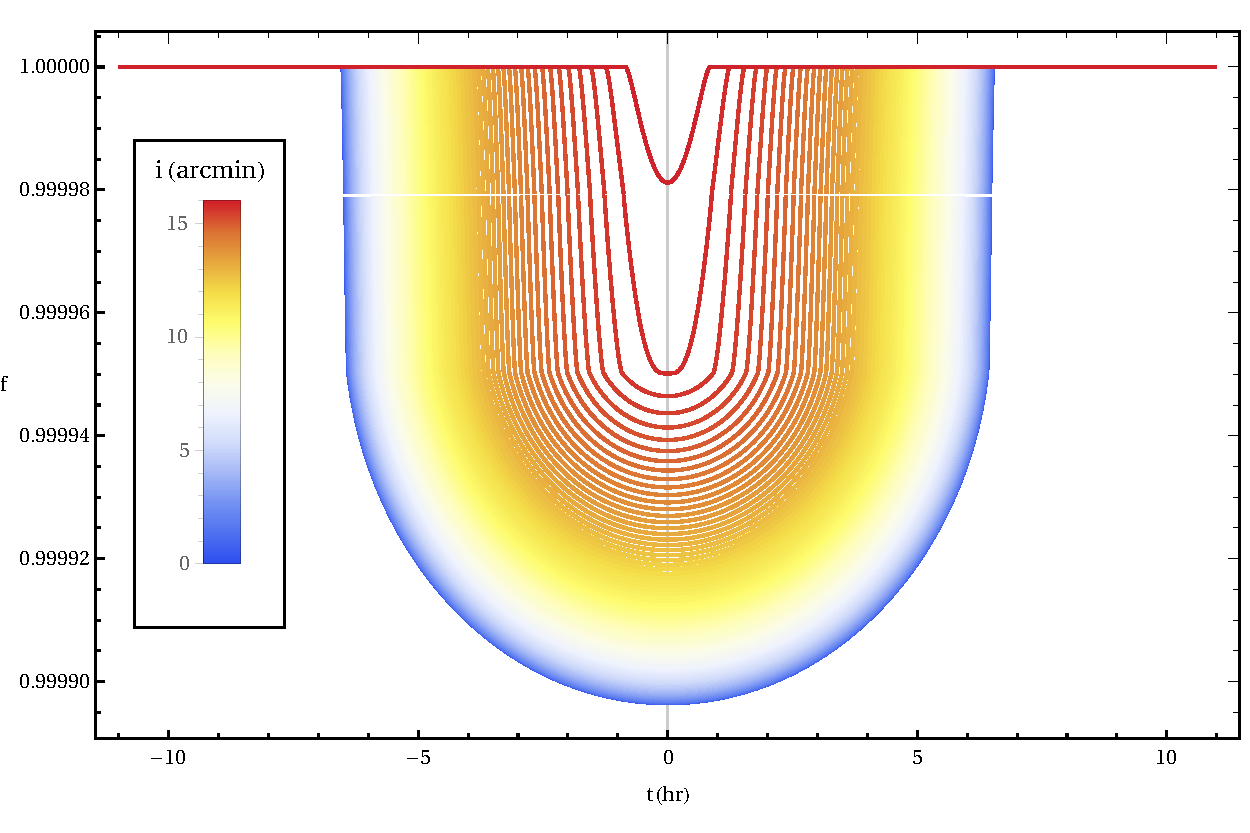
\includegraphics[width=\textwidth]{Planet_Transit_Light_Curve}
    \caption{The flux ratio curves for earth -- sun transits with time measured in hours. The curves vary over orbital inclination.}
\end{figure}
\end{center}


\end{document}